\documentclass[../main.tex]{subfiles}

\begin{document}
    \chapter{Introduction}\label{chap:intro}
    \setcounter{page}{1}

    After many decades of ups and downs, deep learning techniques recently produced unprecedented breakthroughs
    in complex areas like computer vision, speech recognition, and natual language processing. \\
    Deep learning~\cite{deeplearning} is a subset of machine learning based on Artificial Neural Networks---statistical models loosely
    inspired by insights from neuroscience. \\
    Two were the main enablers for this revolution: the ever increasing availability of large labeled
    datasets and the terrific growth of computational power that took place in recent years. In particular,
    the advent of GPUs speeded-up by orders of magnitude the kind of computations needed by deep learning.

    \begin{figure}[h!]
        \centering{}
        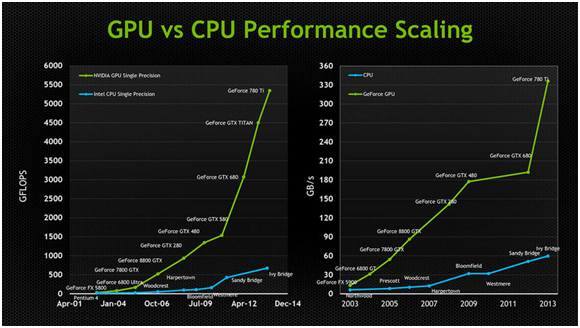
\includegraphics[width=300px]{img/gpu-vs-cpu.png}
        \caption{GPUs are optimized for parallel tasks, thus they are particularly suited to carry out computations
        like matrix multiplication, which is obiquitous in deep learning.}\label{fig:gpu-vs-cpu}
    \end{figure}

    In computer vision in particular, state-of-the-art approaches for tasks such as image recognition,
    object detection and image segmentation all have Convolutional Neural Networks (CNNs)~\cite{lecun-89e} at their core:
	these are a specialization of the more general feedforward network architecture able to deal with data characterized by a grid-like topology.

    Like the majority of machine learning technologies, also deep learning relies on the i.i.d.\ (independent and identically distributed) assumptions~\cite{Vapnik1998}, according to which,
    the training and test samples are drawn
    from the same data generating process, i.e.\ by the same distribution. \\
	The problem of dealing with settings in which the i.i.d.\ assumptions
	do not hold is known as Domain Adaptation~\cite{domain-adaptation-review}, in which we seek to minimize generalization error
	in those situations in which there is a significant shift between the training distribution
    (also called \textit{source domain} in the domain adaptation terminology) and the test distribution (called \textit{target domain}). \\
    Domain adaptation has important practical consequences, as solving this problem would imply being able to train offline models
    on huge dataset, and have them generalize well when deployed on the real-world.
    A typical scenario is that of a mobile app in which users take photos that are to be analyzed (e.g.\ classified, segmented, \ldots) by
    an algorithm. These pictures are likely to come from a different distribution than that of ImageNet~\cite{imagenet} for instance,
    and also are likely to be different between different users.
    The possibility of having a model (trained offline) capable of generalizing to these kinds of situations represents a practical, and
    useful, application of domain adaptation. \\
    In the most recent computer vision literature there has been several attempts to combine deep learning and domain adaptation, however all the used experimental testbeds involve images with objects mainly appearing in the center and the learning procedure consider the images as a whole. In our work we want to deal with more realistic settings like that involved in robotics applications where pictures might be taken from very different angles and viewpoints and the domain shift is caused by significant variations in translation and scale. In these conditions, localizing the image parts more responsible for domain shift when applying the adaptation is highly beneficial. By following this intuition, in this work we propose a tailored adaptive deep learning architecture that outperforms existing baselines. \\
    The rest of the thesis is organized as follows. Chapter~\ref{chap:background} reviews basic concepts of machine learning and in particular summarizes the main elements of deep learning and convolutional neural networks. Chapter~\ref{chap:related} focuses on domain adaptation presenting its main challenges as well as previous literature.
    In~\autoref{chap:approach} we describe our approach, the LoAd (Localized Adaptive) Network, describing
    the main components and the techniques it builds upon. In~\autoref{chap:experiments} and~\autoref{chap:comparison},
    experiments across a variety of robotics datasets and network architectures are reported.
    The thesis concludes with~\autoref{chap:summary} with a summary and a discussion on future research.

\end{document}
